\chapter{DELF}\label{delf_chapter}
Das Delf-Verfahren \cite{delf} von Noh, \mbox{Araujo} et al. bildet die Basis für die Experimente, die in dieser Arbeit durchgeführt werden. Im folgenden Abschnitt wird das Verfahren schrittweise im Detail erklärt. Beschrieben wird hierbei die Neuimplementierung in ihrer Basiskonfiguration, wie sie für den Experimentalteil dieser Arbeit verwendet wird. Unterschiede zu der von den Autoren zu Verfügung gestellten Implementierung\footnote[1]{\url{https://github.com/tensorflow/models/tree/master/research/delf}, zuletzt besucht 16.06.20}, sowie zu der Beschreibung des Verfahrens im Originalpapier \cite{delf} werden im hinteren Teil des Abschnitts erläutert. 
\\\\
Das Delf-Verfahren lässt sich in vier Phasen einteilen. Zu Beginn steht das sogenannte Fine-Tuning. Hierbei wird ein vortrainiertes Modell, in unserem Fall ein ResNet-50 Netzwerk, auf einem neuen Datensatz weiter trainiert. Die Domäne der Bilder dieses Datensatzes sollte dabei möglichst nahe der späteren Retrievalaufgabe sein, damit das Modell lernen kann aussagekräftige Deskriptoren für diese Art von Bilden zu berechnen. In der nächsten Phase wird auf dem Modell aufbauend ein Attention-Netzwerk trainiert welches die Güte berechneter Deskriptoren bewertet. In der dritten Phase werden für die Bilder der Datenbank, in der gesucht werden soll Deskriptoren extrahiert. Mit Hilfe des Attention-Netzwerks wird eine Vorauswahl besonders geeigneter Deskriptoren getroffen. Anschließend durchlaufen die Deskriptoren weitere Vorverarbeitungsschritte, mit denen sie in eine kompaktere Form überführt werden. In der finalen Phase kann Delf aktiv genutzt werden. Es können nun Bilder als Suchanfragen gestellt werden. Delf vergleicht eine Anfrage mit allen Bildern des Datensatzes anhand der vorverarbeiteten Deskriptoren. Potentielle Matches zwischen Deskriptoren werden in einem letzten Schritt geometrisch verifiziert. Das Ergebnis einer Anfrage ist eine Rangliste der ähnlichsten Bilder, sortierte nach der Anzahl verifizierte Deskriptoren-Matches mit dem Anfragebild.

\section{ResNet}

Das Delf-Verfahren nutzt zur Erstellung von Deskriptoren ein Residuales Netzwerk (kurz ResNet). Bei der im Jahre 2015 vorgestellten ResNet Architektur \cite{resnet} von He, Zhang et al. handelt es sich um eine der meist genutzten tiefen CNN-Architekturen der aktuellen Forschung. ResNets finden Anwendung in unterschiedlichen Machine Learning Aufgaben, wie Klassifikation, Objektdetektion oder Image Retrieval. \\

Zeiler und Fergus haben gezeigt \cite{extraction_point_meaning}, dass CNNs mit wachsender Netzwerktiefe in der Lage sind komplexere Merkmale zu detektieren. Es scheint daher intuitiv zur Lösung immer komplexerer Aufgaben zunehmend tiefere Netzwerke zu konstruieren. Allerdings stellt sich heraus, dass ab einem gewissen Punkt keine Verbesserungen mehr mit dem bloßen aneinanderreihen von immer mehr Schichten erzielt werden können. Werden zu viele Schichten hinzugefügt kann die Trainingsperformanz sogar abnehmen. Mit dem rasanten Anstieg der Anzahl an Netzwerkparameter wird es immer schwieriger das Netzwerk zu optimieren. Parameter konvergieren deutlich langsamer zu einem Optimum und es gibt mehr lokale Minima in denen ein Netzwerk im Optimierungsprozess stecken bleiben kann. ResNets wirken diesem Problem mit der Einführung sogenannter Skip-Verbindungen entgegen. Hierbei werden zusätzliche Direktverbindungen im Netzwerk geschaffen, bei denen einige Schichten übersprungen werden. Fließt eine Eingabe an den Beginn einer Skip-Verbindung, so wird auf dieser die Identität der Eingabe mitgeführt. Parallel durchläuft die Eingabe die übersprungenen Schichten. Am Ausgangspunkt der Verbindung wird schließlich die Ausgabe der übersprungenen Schichten mit der Identität aufsummiert (siehe Abb. \ref{resnet}a). Durch die Bereitstellung der Identität hat das Netzwerk eine bessere Grundlage zur Optimierung und einzelne schlecht optimierte Schichten weniger negative Auswirkung auf die Netzwerkausgabe. Die Autoren stellen fest, dass CNNs bei Verwendung von Skip-Verbindung schneller zu einem Optimum konvergieren und dabei bessere Minima gefunden werden. 
\\
ResNets können in unterschiedlichen Konfigurationen erstellt werden. Das für Delf verwendete \mbox{ResNet-50} besteht aus 49 faltenden gefolgt von einer vollvernetzen Schicht. Skip-Verbindungen überspringen jeweils drei Schichten. Das Netzwerk kann in vier Blöcke unterteilt werden. Die Größe der einzelnen Featuremaps, der Ausgabe verringert sich nach jedem Block um den Faktor vier, wohingegen die Merkmalstiefe bzw. Anzahl der Featuremaps in der Ausgabe steigt (Siehe Abb.\ref{resnet}b). In der Implementierung dieser Arbeit wird die von Torchvision zur Verfügung gestellte ResNet-50 Architektur genutzt\footnote[1]{\url{https://github.com/pytorch/vision/blob/c2e8a00885e68ae1200eb6440f540e181d9125de/torchvision/models/resnet.py}, zuletzt besucht 16.06.20}. 
\begin{figure}
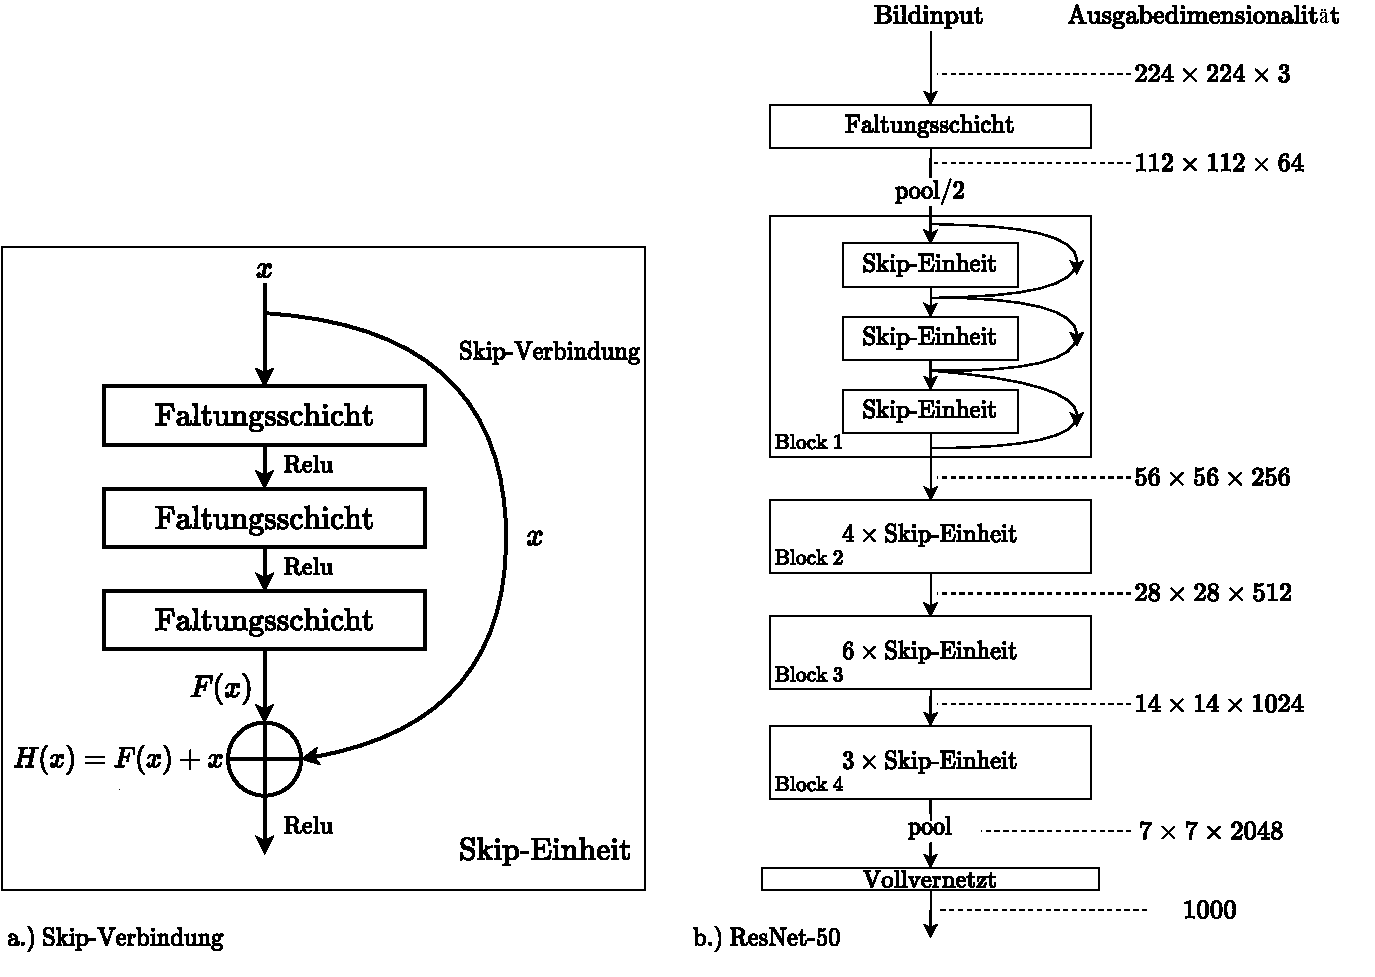
\includegraphics[scale=0.70]{resnet-50.pdf}
\caption{Aufbau der ResNet-Architektur (vgl. Fig.2, Fig.3 aus \cite{resnet})}
\label{resnet}
\end{figure}

\section{Trainingsdaten}
Um die Modelle für das Delf-Verfahren zu trainieren wird ein gelabelter Datensatz benötigt. Zum jetzigen Zeitpunkt steht kein solcher Datensatz von historischen Stadtaufnahmen mit ausreichender Größe zur Verfügung. Für diese Arbeit wird daher alternativ auf die Bilder der Google Landmark Challenge V2 \cite{landmarks_v2} zurückgegriffen. Die Bilder entstammen einer Websuche auf der Wikimedia Datenbank\footnote[1]{\url{https://commons.wikimedia.org}, zuletzt besucht 18.06.20} und zeigen Sehenswürdigkeiten aus der ganzen Welt. Der überwiegende Teil (72\%) zeigt dabei menschengemachte Sehenswürdigkeiten, wie Kirchen, Museen oder Häuser. Auch wenn historische Aufnahmen keinen wesentlichen Teil der Bilder ausmachen enthält der Datensatz viele ähnliche Inhalte zu den historischen Datensätzen, die für das Retrieval genutzt werden. Der Trainingssatz der Landmark Challenge ist mit über 4 Millionen Bildern aus über 200k unterschiedlichen Kategorien sehr groß und heterogen. Da bei der Zusammenstellung keine Verifizierung der Bildinhalts durchgeführt wird kommt es häufig vor, dass Bilder in der falschen Kategorie einsortiert sind. Für das Delf-Training wird daher ein bereinigtes Subset des Datensatzes verwendet, welches von Yokoo, Ozaki et al. in Rahmen ihrer Arbeit \cite{landmarks_verified} erstellt wurde. Aus dem bereinigten Datensatz werden die 40 häufigsten Kategorien gewählt und so ein Trainingsdatensatz über 39\,790 gelabelten Bildern erstellt. 

\section{Fine-Tuning}

Das Ziel der ersten Trainingsphase ist es das ResNet Modell so zu optimieren, dass das Modell bei der Verarbeitung eines Bildes Zwischenergebnisse erzeugt, die den Bildinhalt aussagekräftig beschreiben. Dies ist die Voraussetzung, um später leistungsstarke Deskriptoren erstellen zu können. Während der Optimierung versucht das Netzwerk die Klassifikationsaufgabe des Trainingsdatensatzes zu lösen. Zu Beginn werden die Netzwerkparameter dabei nicht zufällig initialisiert. Stattdessen wird ein Vortrainiertes Modell als Ausgangspunkt genutzt. Diese Art des Trainings wird als Fine-Tuning bezeichnet und ist eine gängige Methode, um den Trainingsprozess zu erleichtern. Auch in anderen Image Retrival Systemen \cite{convnet} \cite{siamac_contrastive_loss} wird diese Art des Trainings genutzt. Zeiler und Fergus zeigen in ihren Experimenten (vgl. \cite{extraction_point_meaning} Kapitel 5.2), dass Netzwerke beim Training lernen allgemein nützliche Merkmale zu extrahieren, die sich auf unterschiedliche Datensätze anwenden lassen. Um ein vortrainiertes Netzwerk auf einen neuen Datensatz anzupassen sind daher nur kleine Veränderungen der Netzwerkparameter notwendig.
\\
Als Ausgangspunkt für das Delf-Training wird ein auf ImageNet trainiertes ResNet-50 genutzt. Bei ImageNet handelt es sich um einen sehr große Klassifikationsdatensatz mit 1.4M Bildern aus 1000 sehr unterschiedlichen Kategorien. Durch die Vielfalt an Kategorien eigenen sich auf ImageNet trainierte Netzwerke als Ausgangspunkt für viele Klassifikationsaufgaben. Daher stellen die meisten Machine Learning Frameworks auf ImageNet trainierte Netzwerke zur Verfügung\footnote[2]{\url{https://pytorch.org/docs/stable/torchvision/models.html}, zuletzt besucht 23.06.20}. 
\\
Während dem Training erwartet das Netzwerk quadratische Bilder mit einer Seitenlänge von 224 Pixeln und 3 Farbkanälen als Eingabe. Hierfür werden die Trainingsdaten zunächst quadratisch zugeschnitten und auf $250\times250$ Pixel skaliert. Anschließend wird ein zufälliger $224\times244$ Pixelbereich ausgewählt.
Um das vortrainierte Netzwerk auf dem Trainingssatz weiter zu trainieren muss das Netzwerk so angepasst werden, dass die Ausgaben der letzten Schicht die korrekte Form für die zur Optimierung verwendete Fehlerfunktion hat. Als Fehlerfunktion wird hier der Cross-Entropy Loss berechnet:
\begin{equation}
\text{CrossEntropyLoss}(Y,\hat{Y}) = -\sum_{\forall c \in C}{Y(c)*\log\hat{Y}(c)}
\end{equation}
$\hat{Y}$ ist hierbei die Verteilung der Klassenwahrscheinlichkeiten, die das Modell für eine Eingabe vorhergesagt hat. $\hat{Y}(c)$ ist die vom Netzwerk bestimmte Wahrscheinlichkeit, mit der die Eingabe der Klasse $c$ zuzuordnen ist. $Y$ beschreibt die tatsächliche Kategorie der Eingabe. $Y$ ist also ein Verteilung, bei der die Wahrscheinlichkeit für jede, bis auf die korrekte Kategorie 0 und für die tatsächliche Klasse 1 ist. Als Ausgabe des Netzwerks wird also ein Vektor der Wahrscheinlichkeitsverteilung erwartet, dessen Dimensionalität der Anzahl der unterschiedlichen Klassen $|C|$ im Datensatz entspricht und dessen Einträge sich auf 1 summieren. \\
Damit die Ausgaben des Netzwerks die richtige Dimensionalität haben wird zunächst die letzte vollvernetzte Schicht entfernt. An ihre Stelle tritt eine faltenden Schicht mit $1\times1$ Filtermasken, die eine Merkmalstiefe von $2048$ erwarten, was der Dimensionalität vorangehenden Schicht entspricht (vgl. Abb. \ref{resnet}b). In der faltenden Schicht werden $|C|$ dieser Filtermasken auf die Eingabe angewendet, wodurch die Ausgabe die gewünschte Dimensionalität erhält.
Um die Netzwerkausgaben in den richtigen Wertebereich zu überführen, werden diese von einer Softmaxfunktion aktiviert, bevor die Fehlerfunktion berechnet wird:
\begin{equation}
\text{Softmax}(\hat{Y'})_{c} = \frac{e^{\hat{Y'_c}}}{\sum_{\forall x \in C}{e^{\hat{Y'_x}}}} \forall c \in C
\end{equation}
Hierbei ist $\hat{Y'}$ ein Ausgabevektor des Netzwerks und $\hat{Y'_c}$ der Eintrag des Vektors welcher zur Klasse $c$ zugeordnet ist. Der resultierende Vektor kann als Wahrscheinlichkeitsverteilung über die unterschiedlichen Klassen im Bezug zur Eingabe interpretiert werden. Mit den vorgenommenen Modifikationen kann das ResNet Modell auf dem Trainingsdatensatz optimiert werden. Die für das Fine-Tuning und Attention-Training verwendeten Hyperparamter werden im Experimentalteil in Sektion \ref{hyperparam} erläutert.

\section{Attention Training}

Delf erzeugt eine große Anzahl an lokalen Deskriptoren, um Bilder zu beschreiben. Da jeder Deskriptor nur einen Ausschnitt des Originalbildes beschreibt, werden auch Deskriptoren für wenig aussagekräftige Bereiche, wie z.B. Teile des Himmels erstellt. Diese Deskriptoren beanspruchen nicht nur zusätzliche Rechenzeit während des Matchingprozesses sondern können auch zu falsch positiven Matches führen. Ziel der zweiten Trainingsphase ist es daher auf Basis dieser Deskriptoren ein Netzwerk zu trainieren, welches in der Lage ist die Qualität der Deskriptoren zu bewerten und so ungeeignete Kandidaten herauszufiltern. 
Zur Erstellung der Deskriptoren dient das ResNet-50, welches in der ersten Phase trainiert wurde. Als Deskriptoren werden dabei die Ausgaben aus dem dritten ResNet-Blocks genutzt (vgl. Abb. \ref{resnet}b). Die Ausgaben haben eine Dimensionalität von $w\times h\times 1024$, wobei $w$ und $h$ abhängig von der Breite und Höhe des Eingabebildes sind. Die einzelnen Koordinaten der $1024$ Featuremaps lassen sich jeweils auf einen Bildbereich in der Eingabe zurückführen. So kann die Ausgabe in $w \times h$ Deskriptoren der Größe $1024$ eingeteilt werden. Wie auch beim Fine-Tuning werden die Bilder für das Training zunächst quadratisch zugeschnitten. Anschließend werden sie auf eine zufällige Seitenlänge zwischen $255$ bis $720$ Pixel skaliert. Die Skalierung hat Einfluss auf die Beschaffenheit der entstehenden Deskriptoren. Durch das zufällige Skalieren der Trainingsbilder lernt das Attention-Netzwerk mit Deskriptoren aus verschiedenen Skalen umzugehen. Während dem Attention-Training werden die Parameter des ResNets nicht mehr verändert. Die Schichten nach dem Extraktionspunkt in Block 3 werden nicht mehr benötigt und können verworfen werden. \\
Aufgabe des Attention-Netzwerks ist es für eine Eingabe an Deskriptoren der Form $w\times h\times 1024$ eine einzelne Featuremap der Größe $w\times h$ zu generieren, dessen Werte jeweils einen Deskriptor bewerten. Wichtig ist dabei, dass die Berechnung der einzelnen Attention-Werte nur von den Werte der dazugehörigen Deskriptoren abhängen dürfen. Dies kann durch faltenden Schichten mit $1\times1$-Filtermasken realisiert werden. Die Attention-Einheit besteht aus zwei solcher Schichten, welche die Merkmalstiefe der Deskriptoren sukzessive auf $1$ reduzieren (vgl. Abb. \ref{attention}a).  
\begin{figure}
\centering
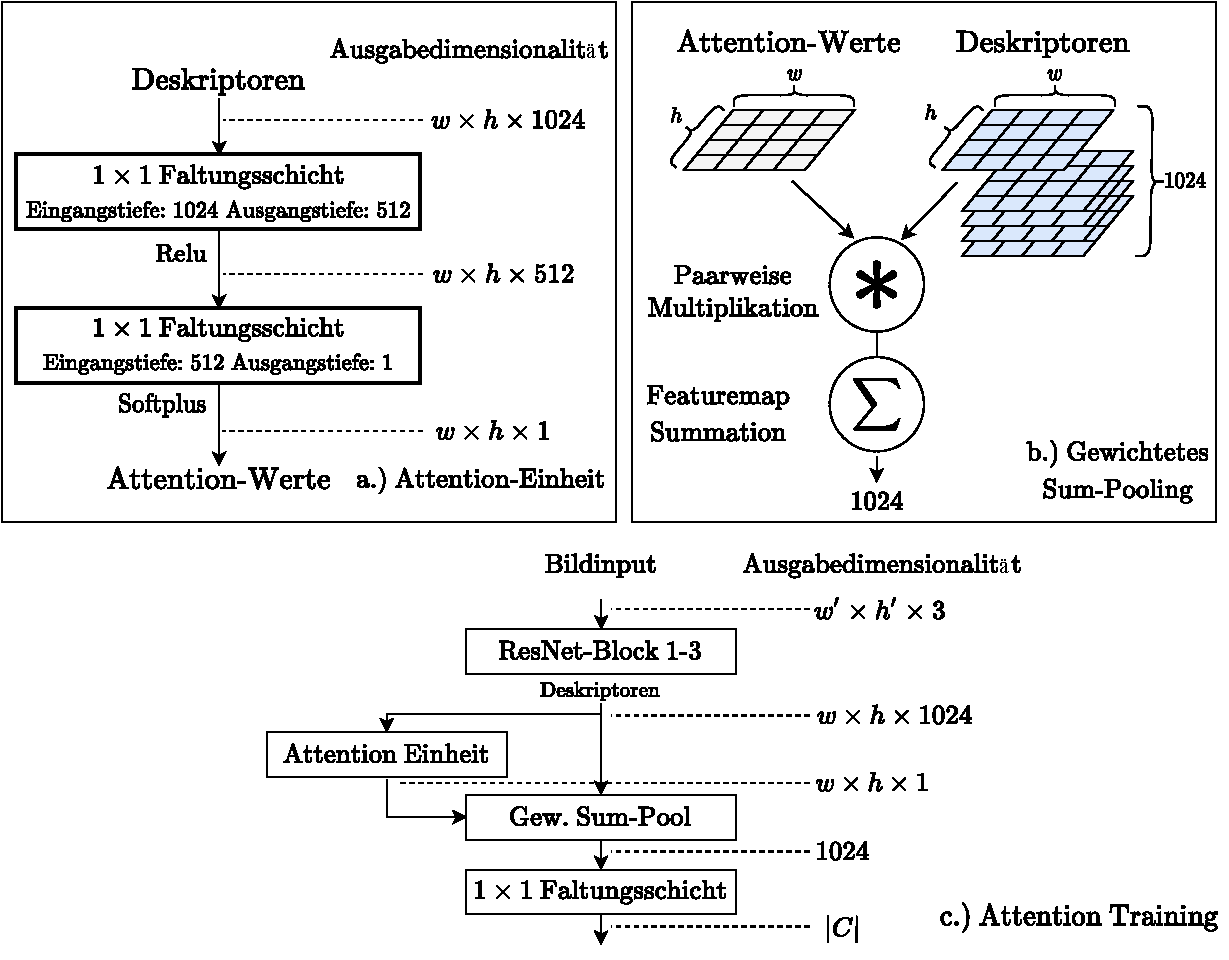
\includegraphics[scale=0.77]{attention_spaced.pdf}
\caption{Architektur des Attention Trainings}
\label{attention}
\end{figure}
Um die Parameter der Attention-Einheit zu optimieren müssen ihre Ausgaben zur Lösung der Trainingsaufgabe beitragen. Da die Attention-Werte später genutzt werden um zu entscheiden, welche Deskriptoren Einfluss auf die Lösung der Retrievalaufgabe haben ist es sinnvoll sie auch beim Training in einer Form zu nutzen, die den Einfluss der Deskriptoren zur Lösung der Klassifikationsaufgabe reguliert. Die Attention-Werte werden zur Gewichtung der Deskriptoren genutzt und dafür elementweise mit den Featuremaps der Deskriptoren Multipliziert. Anschließend werden die gewichteten Featuremaps zu jeweils einem Wert aufsummiert. Als Ausgabe ergibt sich ein $1024$ dimensionaler Vektor (vgl. Abb. \ref{attention}b). Abschließend muss die Ausgabe in eine passende Form für die Cross-Entropy Loss Fehlerfunktion gebracht werden. Dies geschieht analog wie im Fine-Tuning durch Verwendung einer $1\times1$-Faltungsschicht und anschließender Softmaxaktivierung der Ausgabe (vgl. \ref{attention}c).

\section{Extraktion und Verarbeitung}

Nachdem das Training der Modelle abgeschlossen ist, kann mit der Extraktion aller benötigten Informationen über den Retrievaldatensatz begonnen werden. Netzwerkparameter werden ab jetzt nicht mehr modifiziert. Schichten und Operationen nach der Attention-Einheit erfüllen daher keine Zweck mehr und können entfernt werden.
\subsection{Multi-Skalen-Extraktion}
Für jedes Bild des Retrievaldatensatzes werden die lokalen Deskriptoren am Extraktionspunkt nach dem dritten ResNet-Block und die dazugehörigen Attention-Werte nach der Attention-Einheit extrahiert. Da die Skalierung des Bildinhalts Einfluss auf die resultierenden Deskriptoren hat, wird für jedes Bild eine Reihen von unterschiedlich skalierten Versionen betrachtet. Dies ist vergleichbar mit der Verwendung des Scale Spaces im SIFT-Verfahren (vgl. Kap.\ref{related_work} Abs.2) und soll zur Invarianz gegenüber Skalierungsoperationen beitragen. Für jedes Bild werden sechs unterschiedlichen Skalen mit Skalierungsfaktoren zwischen $2$ und $\frac{1}{4}$ erstellt, wobei sich benachbarte Skalen um den Faktor $\sqrt{2}$ unterscheiden. 
\subsection{Deskriptorlokalisierung}
Für den weiteren Verlauf des Verfahrens muss jeder lokale Deskriptor einem Bereich des Eingangsbildes zuortbar sein. Bei allen verwendeten Schichten des Modells bis zum Extraktionspunkt handelt es sich um Faltungs- oder Poolingschichten. Von welchen Bereichen der Eingabe die Ausgaben dieser Schichten abhängen lässt sich an drei Parametern festmachen. Die Größe der Filtermasken $k$ bestimmt die Größe des Einflussbereiches einzelner Ausgaben. Die Verschiebung der Filtermasken bzw. die Schrittgröße $s$ bestimmt die Verschiebung zwischen den Einflussbereichen benachbarter Ausgaben. Das Padding $p$ bestimmt die Größe des Pufferbereichs, der der Eingabe hinzugefügt wird, und sorgt so für eine initiale Verschiebung der Einflussbereiche. Das Padding ist im folgenden immer symmetrisch und wird daher an jeder Seite der Eingabe hinzugefügt. Betrachtet man mehrere aufeinanderfolgende Schichten, so lassen sich die Einflüsse dieser Parameter wie folgt rekursiv berechnen:
\begin{align}
\hat{k}_n &= \hat{k}_{n-1} + ((k_n - 1) * \hat{s}_{n-1})
\\
\hat{s}_n &= \hat{s}_{n-1} * s_n
\\
\hat{p}_n &= \hat{p}_{n-1} + (p_n * \hat{s}_{n-1})
\\
\hat{k}_0 &= k_0
\\
\hat{s}_0 &= s_0
\\
\hat{p}_0 &= p_0
\end{align}
Wobei $\hat{k}_n$, $\hat{s}_n$ und $\hat{p}_n$ die Größe der Einflussbereiche, Schrittgröße und Paddinggröße im Bezug zur ursprüngliche Eingabe nach $n$ Schichten repräsentieren. $k_n$, $s_n$ und $p_n$ zeigen die selben Größen für Schicht $n$ im Bezug zur Ausgabe der vorangehenden Schicht. In Abbildung \ref{receptive_field} werden diese Berechnungen exemplarisch erklärt. 
\begin{figure}
\centering
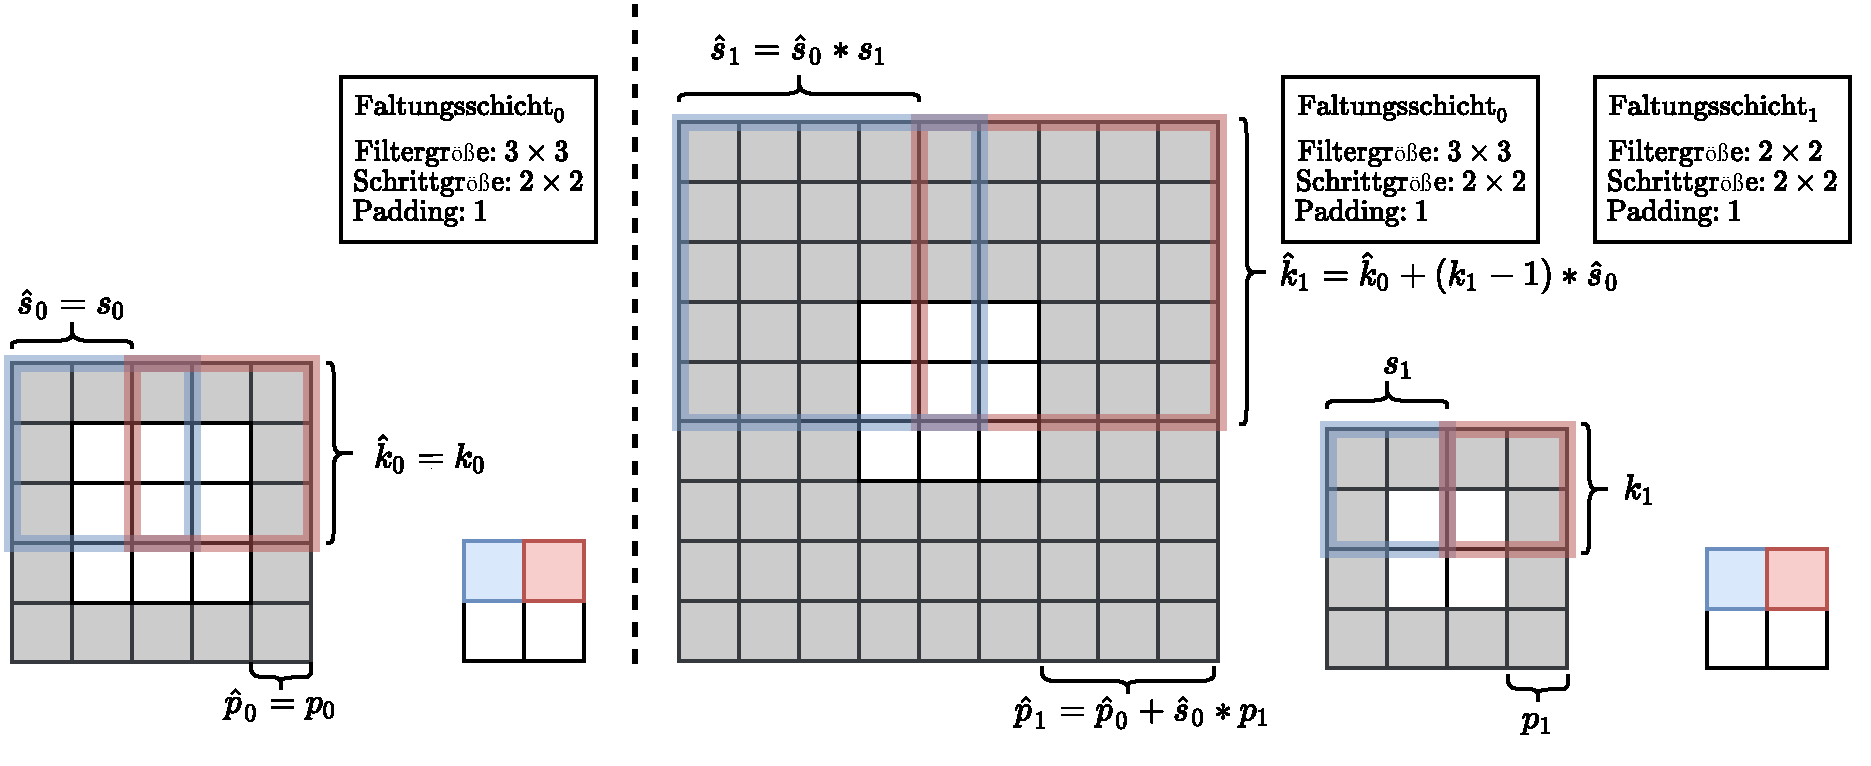
\includegraphics[scale=0.51]{rf.pdf}
\caption{Berechnung des Einflussbereichs einzelner Ausgaben in der ursprünglichen Eingabe. Links nach einer Faltungsschicht, Rechts nach zwei Schichten. Graue Bereiche repräsentiert hinzugefügten Puffer.}
\label{receptive_field}
\end{figure}
Berechnet man diese Werte für den Extraktionspunkt nach dem dritten ResNet-Block ergibt sich für jeden lokalen Deskriptor ein quadratischer Einflussbereich $\mathbf{k}$ mit einer Seitenlänge von $267$ Pixeln im Ursprungsbild. Die Verschiebung zwischen Einflussbereichen benachbarter Deskriptoren $\mathbf{s}$ beträgt dabei $16$ Pixel. Das Ursprungbild erhält bis zu dieser Schicht ein effektives Padding $\mathbf{p}$ von $133$ Pixeln in jede Richtung. Aufgrund dieser Werte lassen sich die Einflussbereiche für alle $w \times h$ Deskriptoren, die am Extraktionspunkt anfallen wie folgt berechnen:
\begin{align}
x_{min}(i,j) &= i*\mathbf{s} - \mathbf{p} 
\\
x_{max}(i,j) &= x_{min}(i,j) + \mathbf{k}
\\ 
y_{min}(i,j) &= j*\mathbf{s} - \mathbf{p}
\\ 
y_{max}(i,j) &= y_{min}(i,j) + \mathbf{k} \qquad\text{ wobei } 0\leq i < w \text{ und } 0\leq j < h
\end{align}

\subsection{Deskriptorselektion}
Im nächsten Verarbeitungsschritt werden die aussagekräftigsten lokalen Deskriptoren auf Basis der Attention-Werte selektiert. Da während der Deskriptorextraktion unterschiedliche skalierte Bildversionen betrachtet wurden steht vor der Selektion ein große Anzahl an Deskriptoren zur Auswahl, die teilweise auch stark überlappende Bildbereiche beschreiben. Das kann dazu führen, dass aus einigen Bildbereichen sehr viele Deskriptoren ausgewählt werden, die zwar individuell viel Information über das Bild bereitstellen, in der Summe aber wenig Nutzen haben, da der gleiche Bildbereich vielfach beschrieben wird. Da die Anzahl der selektierten Deskriptoren pro Bild begrenzt ist, kann dies zu einer Verdrängung von Deskriptoren aus anderen wichtigen Bildbereichen führen. Um dem entgegenzuwirken werden zunächst Deskriptoren, die stark überlappende Bildbereiche beschreiben mittels Non-Maximum-Suppression aussortiert. Als Metrik für die Überlappung wird hierfür die Intersection-over-Union(IoU) zwischen den Einflussbereichen der Deskriptoren berechnet. Also das Verhältnis zwischen überlappenden Flächeninhalt zu gemeinsam eingenommenem Flächeninhalt der Einflussbereiche.
\begin{equation}
\text{IoU}(e_1,e_2) = \frac{e_1 \cap e_2}{e_1 \cup e_2}
\end{equation}
Wobei $e_1$ und $e_2$ Einflussbereiche zweier Deskriptoren sind. Der Non-Maximum-Suppression Algorithmus (siehe Alg. \ref{nms}) erhält als Eingabe eine Liste mit den Einflussbereichen der lokalen Deskriptoren $\mathcal{E}$, die dazugehörigen Attention-Werte $\mathcal{A}$, sowie einen Schwellwert $T$ der maximal tolerierten IoU zwischen den Einflussbereichen der Deskriptoren. Zunächst werden die Kandidaten nach Attention-Wert sortiert. Der Einflussbereich mit dem höchsten Attention-Wert wird ausgewählt und von der Kandidatenliste in die Ergebnisliste geschoben. Anschließend wir die IoU zwischen dem ausgewählten Einflussbereich und den übrigen Einflussbereichen der Kandidatenliste berechnet. Kandidaten dessen IoU den Schwellwert $T$ überschreiten werden aus der Kandidatenliste entfernt. Anschließend wird aus der Kandidatenliste erneut der Einflussbereich mit dem nun höchsten Attention-Wert ausgewählt und der Prozess wiederholt, bis die Kandidatenliste leer ist. Abschließend wird die Ergebnisliste mit den ausgewählten Bereichen und dazugehörigen Attention-Werten zurückgegeben.

\begin{algorithm}
\caption{Non-Maximum-Suppression}
\label{nms}
\DontPrintSemicolon
\KwIn{$\mathcal{E} \leftarrow \{e_1,\ldots,e_n\}$, $\mathcal{A} \leftarrow \{a_1,\ldots,a_n\}$, $T$}
$\mathcal{S} \leftarrow \emptyset$ \;
 \While{$\mathcal{E} \neq \emptyset$}{
  $x \leftarrow$ argmax($\mathcal{A}$) \tcp*[f]{Wähle bestbewertete Box }\;
  $currBox \leftarrow e_x$  \;
  $\mathcal{E} \leftarrow \mathcal{E}\, \backslash \{e_x\}$ \tcp*[f]{Verschiebe Box von Kandidaten in Ergebnisliste} \;
  $\mathcal{A} \leftarrow \mathcal{A}\, \backslash \{a_x\}$ \;
  $\mathcal{S} \leftarrow \mathcal{S} \cup \{(e_x,a_x)\}$ \;
  \ForEach{$e_i \in \mathcal{E}$}
  {\tcp*[f]{Entferne Boxen mit IoU > T zu currBox aus Kandidatenliste} \;
   \If{$\text{IoU}(e_i,currBox) > T$}{ 
   $\mathcal{E} \leftarrow \mathcal{E}\, \backslash \{e_i\}$ \;
   $\mathcal{A} \leftarrow \mathcal{A}\, \backslash \{a_i\}$ \;
   }
   }
 }
 \Return{$\mathcal{S}$}

\end{algorithm}
Im Delf-Verfahren wird für die Vorsortierung ein IoU-Schwellwert von $0.8$ genutzt. Nach der Vorsortierung findet die finale Selektion der Deskriptoren statt. Für jedes Bild werden hierbei von den verbliebenen Deskriptoren die 1000 Deskriptoren mit den höchsten Attention-Werten ausgewählt.

\subsection{Datentransformation und Dimensionsreduktion}

Ziel des letzten Vorverarbeitungsschritts ist es die Daten der lokalen Deskriptoren in eine Form zu bringen, die ein effizientes Vergleichen möglich macht. Obwohl durch den Selektionsprozess bereits die Anzahl an lokalen Deskriptoren je Bild drastisch reduziert wurde ist die aktuelle Repräsentation der einzelnen Bilder noch sehr groß. Mit $1000$ Deskriptoren mit je $1024$ Dimensionen umfasst die Beschreibung jedes Bildes über eine Millionen Werte. Durch die folgenden Transformationen, wird die Größe der lokalen Deskriptoren und damit der gesamt Repräsentation stark reduziert. Die für Delf beschriebenen Transformationen bezeichnen die Autoren dabei als "common practice" (vgl. \cite{delf} Kap.4.3) und beziehen sich dabei auf das von Jégou und Chum in \cite{common_practice} untersuchte Vorgehen zur Transformation von VLAD und BOW-Deskriptoren. Tatsächlich werden Deskriptoren auch in anderen Image Retrieval Verfahren \cite{convnet} \cite{one} auf ähnliche Weise verarbeitet.
\\
Zunächst werden die Deskriptoren der Länge nach normiert. Anschließend wird auf ihnen eine Hauptkomponentenanalyse durchgeführt. Die resultierende Transformationsmatrix soll dabei repräsentative für die Deskriptoren des gesamten Datensatzes sein, daher werden bei der Analyse Deskriptoren des ganzen Datensatzes oder zumindest eines erheblichen Teils betrachtet. Ziel der Hauptkomponentenanalyse ist es die Daten anhand neuer Dimensionen, den sogenannten Hauptkomponenten, darzustellen. Die Richtungen der Hauptkomponenten ergeben sich aus einer Linearkombination der bisherigen Dimensionen und sind so gewählt, dass für die transformierten Daten keine Korrelation zwischen den Dimensionen besteht. Eine weitere Eigenschaft dieser Darstellung ist, dass die einzelnen Hauptkomponenten jeweils den größtmöglichen Anteil, der in den Daten vorhandenen Varianz abbilden. D.h. die Hauptkomponente, die den größten Teil der Varianz abbildet ist die Richtung entlang welcher die Daten am stärksten Variieren. Die Hauptkomponente, die den nächst größten Anteil der Varianz erklärt beschreibt den größtmöglichen Anteil der verbleibenden Varianz. Dies führt dazu, dass der wesentliche Teil der Varianz von wenigen Dimensionen erklärt wird. Dadurch ist es möglich einen großen Teil der Dimensionen zu entfernen, ohne einen starken Informationsverlust zu erleiden.
\\
Sei $X_{n\times d}$ eine Matrix von $n$ zu analysierenden Deskriptoren mit je $d$ Dimensionen. 
Zunächst werden die Daten zentriert, sodass ihr Mittelwert entlang der $d$ Dimensionen $0$ ist:
\begin{equation}
x'(i,j) = \frac{x(i,j)}{\frac{1}{n}\sum_{k=1}^n{x(k,j)}}\qquad \text{für }0<i\leq n\text{, }0<j\leq d
\end{equation}
% 
Häufig werden die Daten anschließend durch die Standardabweichung der einzelnen Dimensionen geteilt um die Varianz je Dimension auf 1 zu setzten. Je größer die Varianz in den Dimensionen ist, desto größer ihr Anteil in den berechneten Hauptkomponenten. Diese Standardisierung wird daher durchgeführt, wenn die Größe der Varianzen der ursprünglichen Dimensionen nicht adäquat ihre Bedeutsamkeit widerspiegeln. Für Delf wird keine Anpassung der Varianz durchgeführt.
%
\\
Im nächsten Schritt wird für die zentrierten Daten $X'_{n \times d}$ die Kovarianzmatrix $C$ berechnet. 
\begin{equation}
C_{d\times d} =  \frac{X^\intercal_{d \times n} * X_{n \times d}}{n}
\end{equation}
Diese lässt sich über Eingenwertzerlegung in ihre Eingenvektoren und Eigenwerte zerlegen.
\begin{equation}
C_{d\times d} = U_{d\times d}\Lambda_{d\times d}U_{d\times d}^\intercal
\end{equation}
$U$ enthält dabei in ihren Spalten die Eigenvektoren von $C$. $\Lambda$ ist eine Diagonalmatrix, die die dazugehörigen Eigenwerte enthält. Die Eigenvektoren geben die Richtungen der Hauptkomponenten an und die dazugehörigen Eigenwerte die Varianz, die durch dich jeweiligen Hauptkomponenten erklärt werden. Sortiert man die Eigenvektoren anhand ihrer Eigenwerte erhält man eine Transformationsmatrix $U'$, mit der sich die Daten so in den Raum der Hauptkomponenten überführen lassen, dass die Dimensionen nach der von ihnen erklärten Varianz sortiert sind. 
\begin{equation}
\hat{X}_{n \times d} = X'_{n \times d} * U'_{d \times d}
\end{equation}
Verkürzt man die Transformationsmatrix auf die ersten $k$ Spalten, so werden die Daten in einen $k$-dimensionalen Raum abgebildet.
\begin{equation}
\hat{X}_{n \times k} = X'_{n \times d} * U'_{d \times k}
\end{equation}
In der Delf-Pipeline werden standardmäßig 40 Hauptkomponenten erhalten. In Kapitel \ref{pca_experiments} wird dieser Parameter experimentell untersucht. 
Delf sieht es vor die Deskriptordaten ebenfalls zu weißen, d.h. in eine Form zu bringen, in der zwischen den Dimensionen keine Korrelation herrscht und die Varianz entlang der Dimensionen je 1 beträgt. Die erste Voraussetzung ist dabei durch die Hauptkomponentenanalyse automatisch erfüllt. Für die Anpassung der Varianz müssen die Daten durch die Standardabweichungen der Dimensionen geteilt werden. Dies kann wie Folgt durch Nutzung der Eigenwerte erreicht werden:
\begin{equation}
\hat{X}_{white} = \Lambda^{-1/2}\hat{X}
\end{equation}
Abschließend werden die transformierten Deskriptoren erneut L2-normiert.